% \begin{figure*}[h]%



% \subfigure[\hspace{10pt}($\uparrow\theta_{min}$, $\phi_{min}$): 32\% accuracy, Baseline]{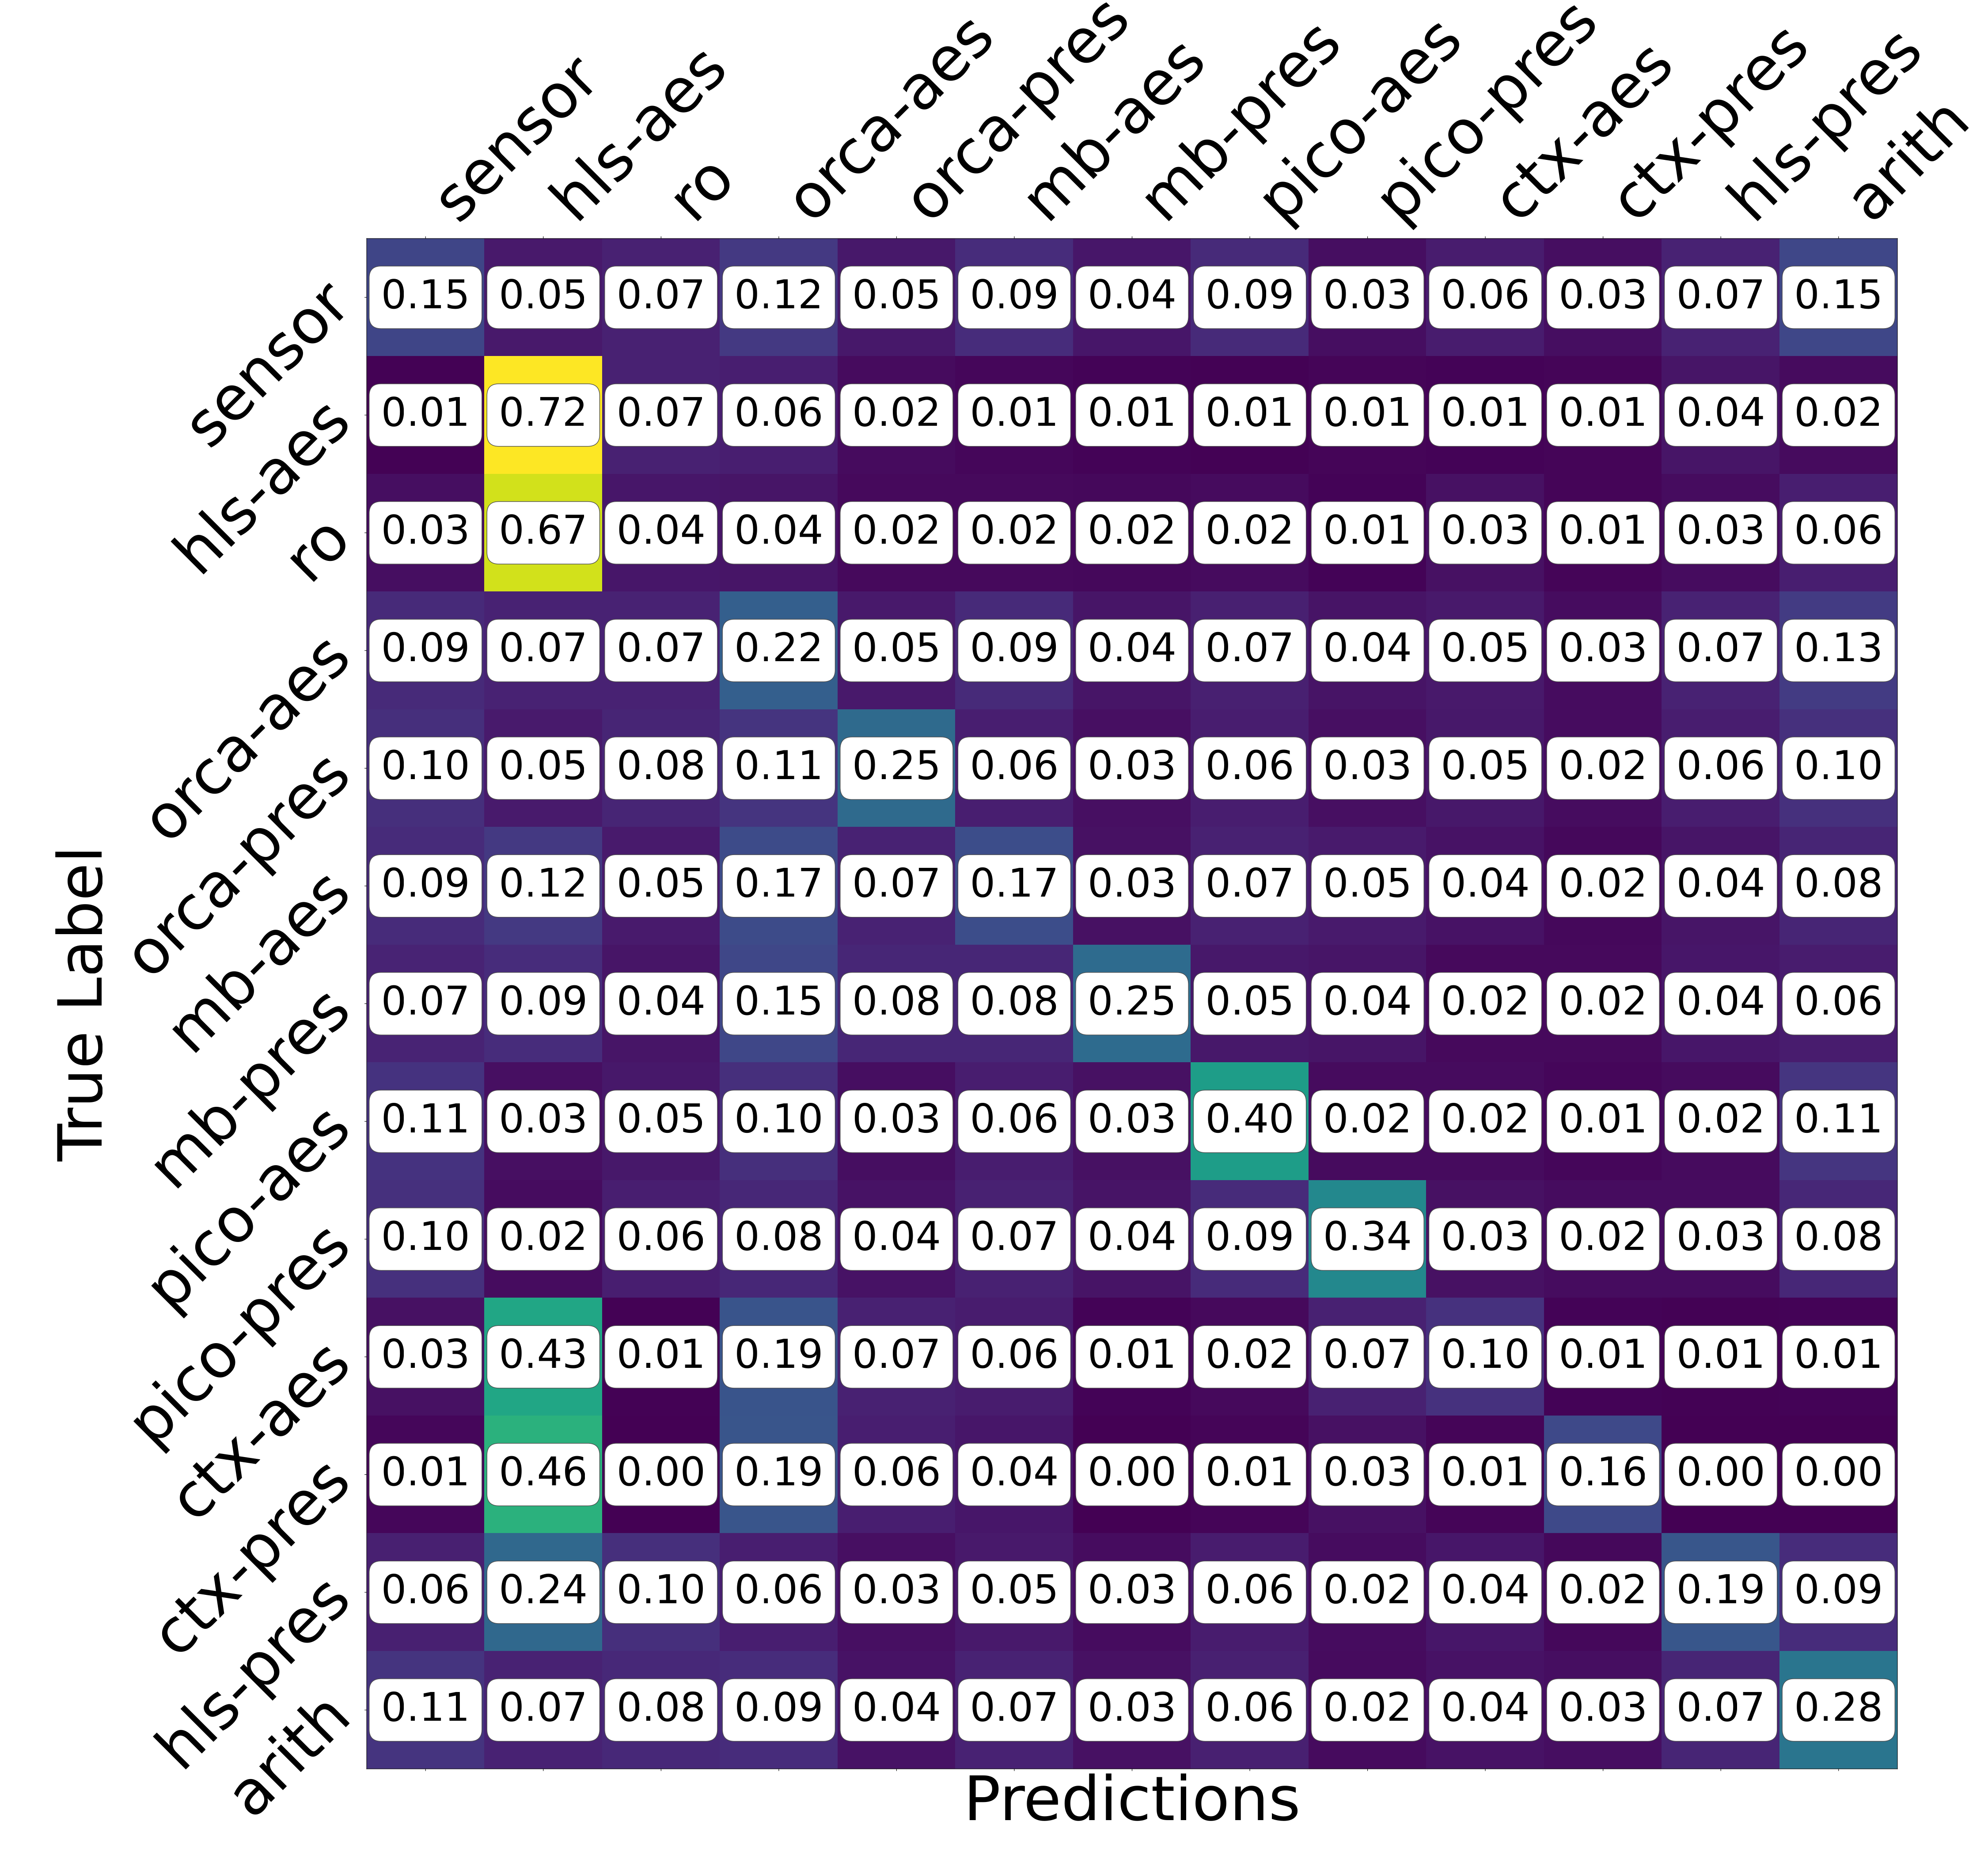
\includegraphics[width=0.45\linewidth]{img/pos-minphi-mintheta-test-board_2e-big-text-confusion-matrix_trimmed.png}\label{classification/rising_min_min}}

% \subfigure[\hspace{10pt}($\downarrow\theta_{max}$, $\phi_{min}$): 51\% accuracy, 1.6$\times$]{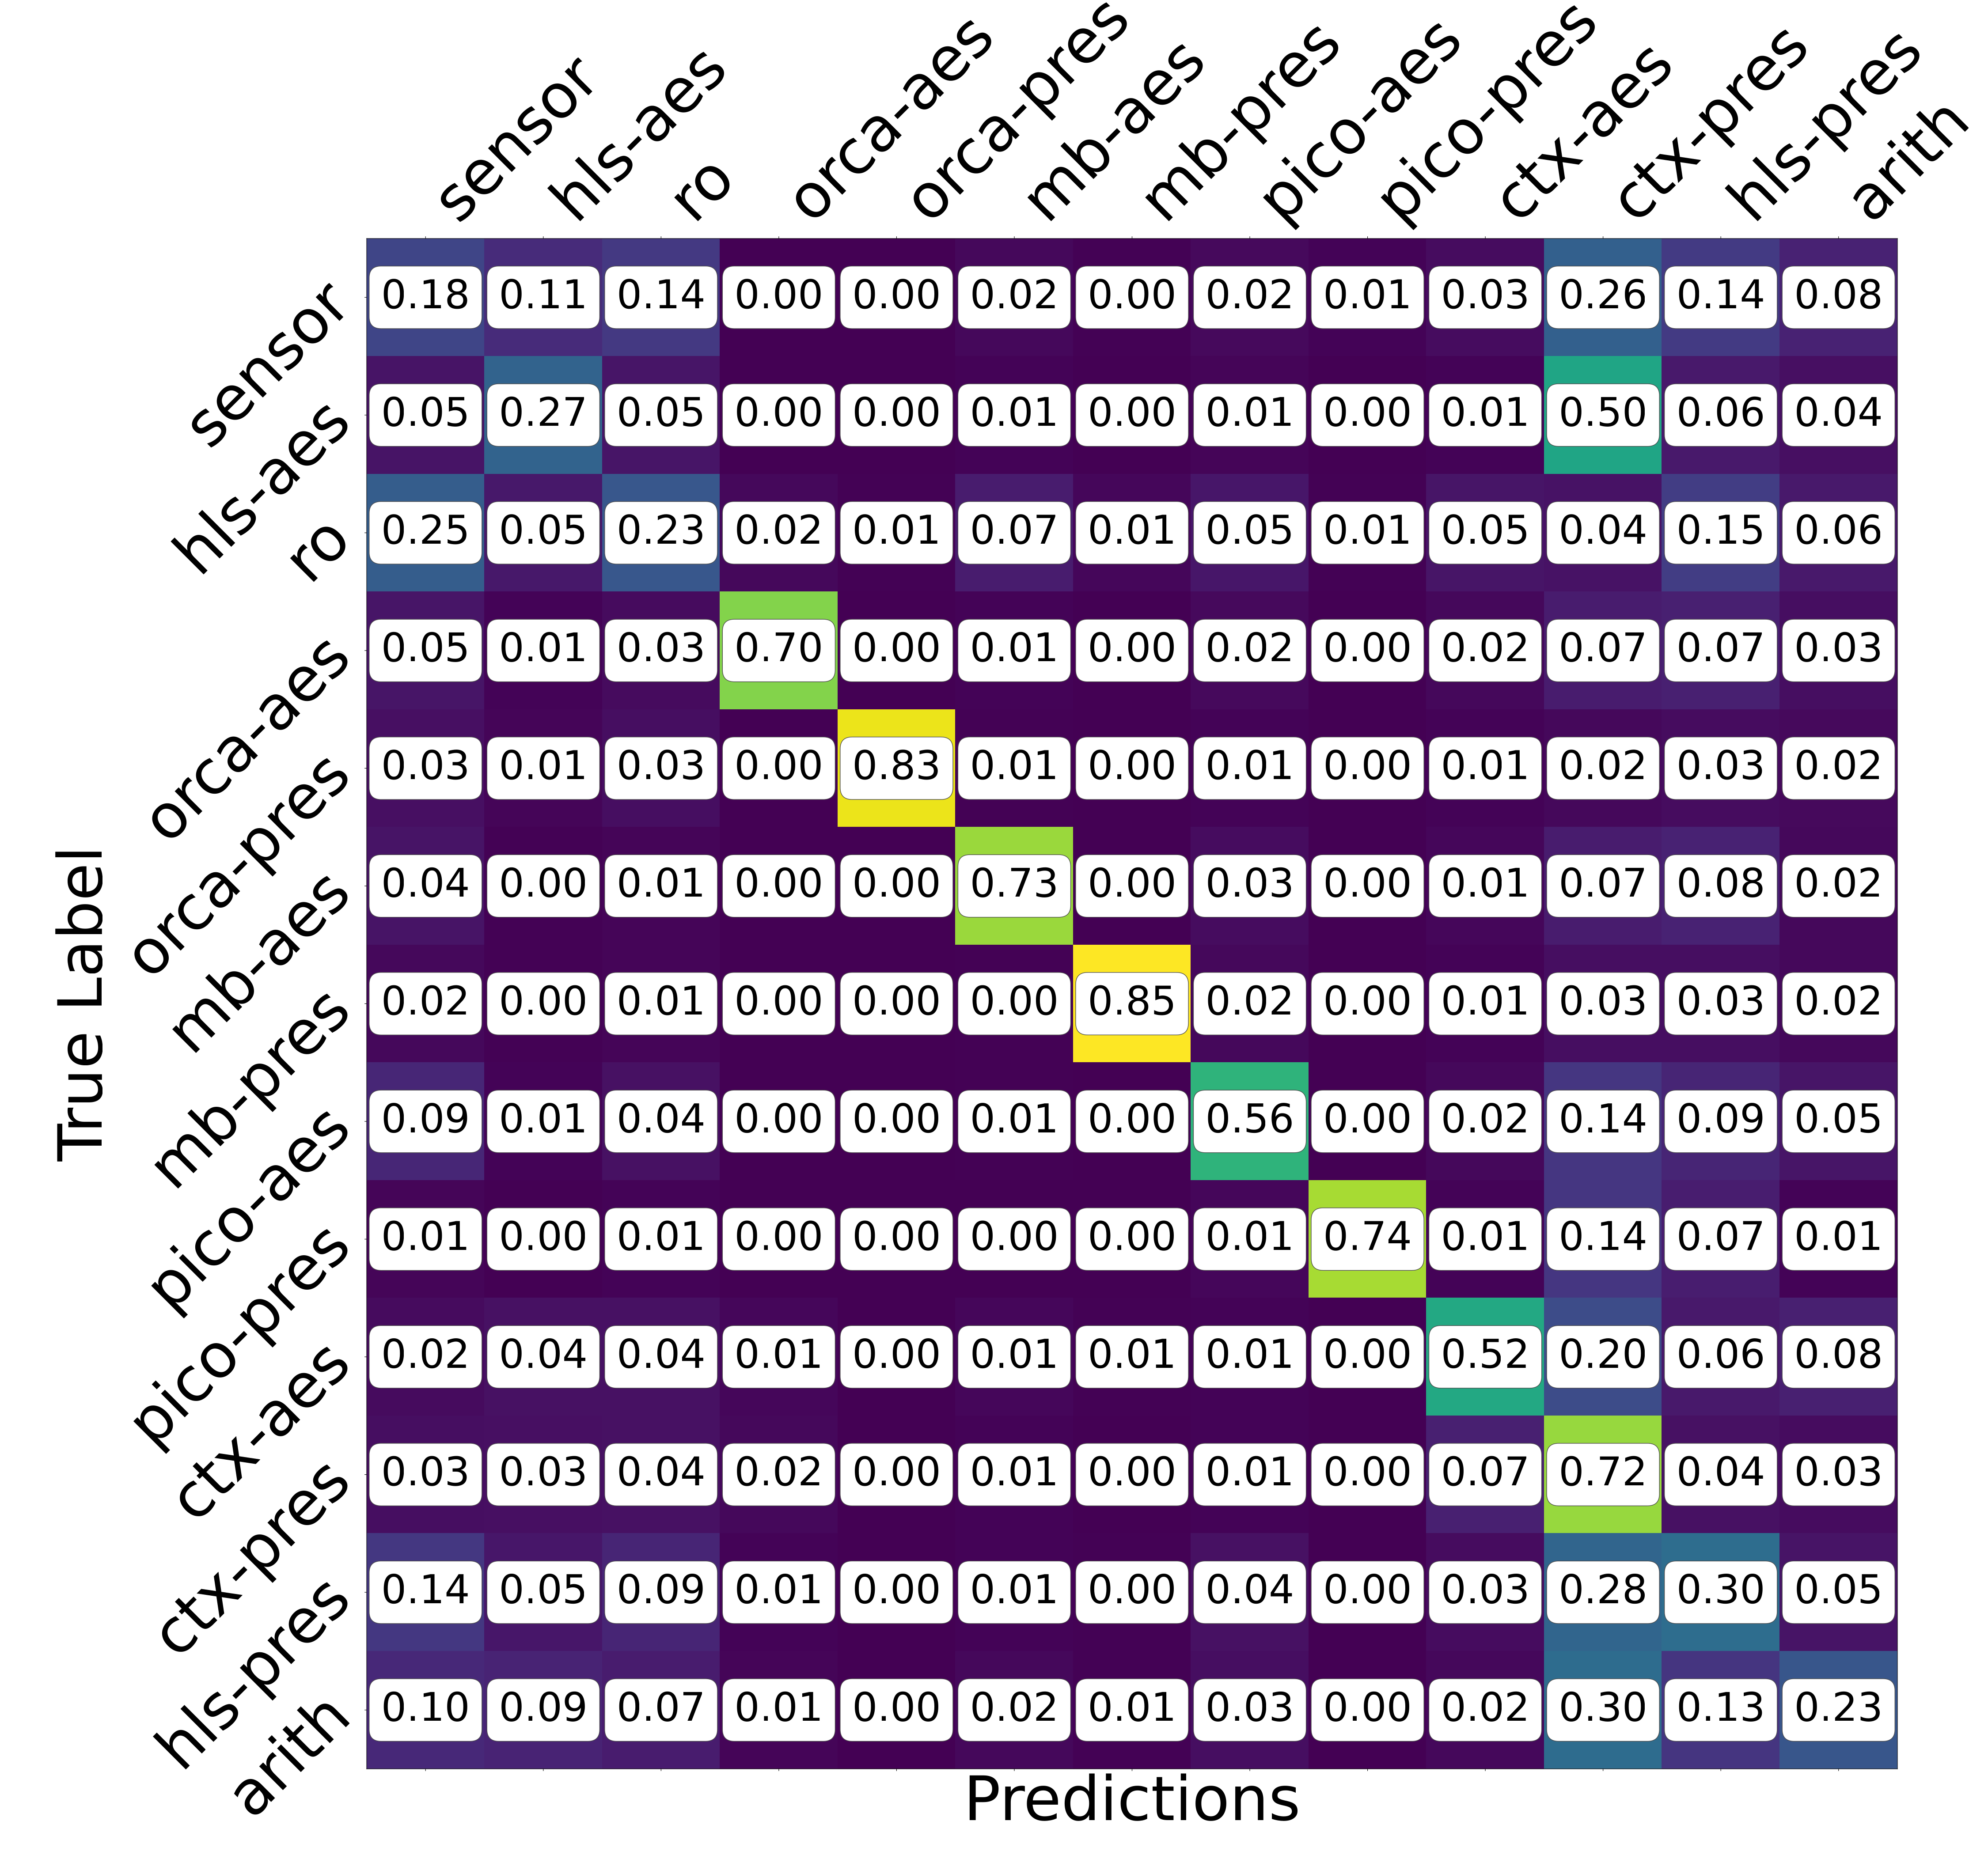
\includegraphics[width=0.45\linewidth]{img/neg-minphi-mintheta-test-board_2e-big-text-confusion-matrix_trimmed.png}\label{classification/falling_min_max}}

% \subfigure[b][\hspace{10pt}($\downarrow\theta_{max}$, $\phi_{back}$): 75\% accuracy, 2.3$\times$]{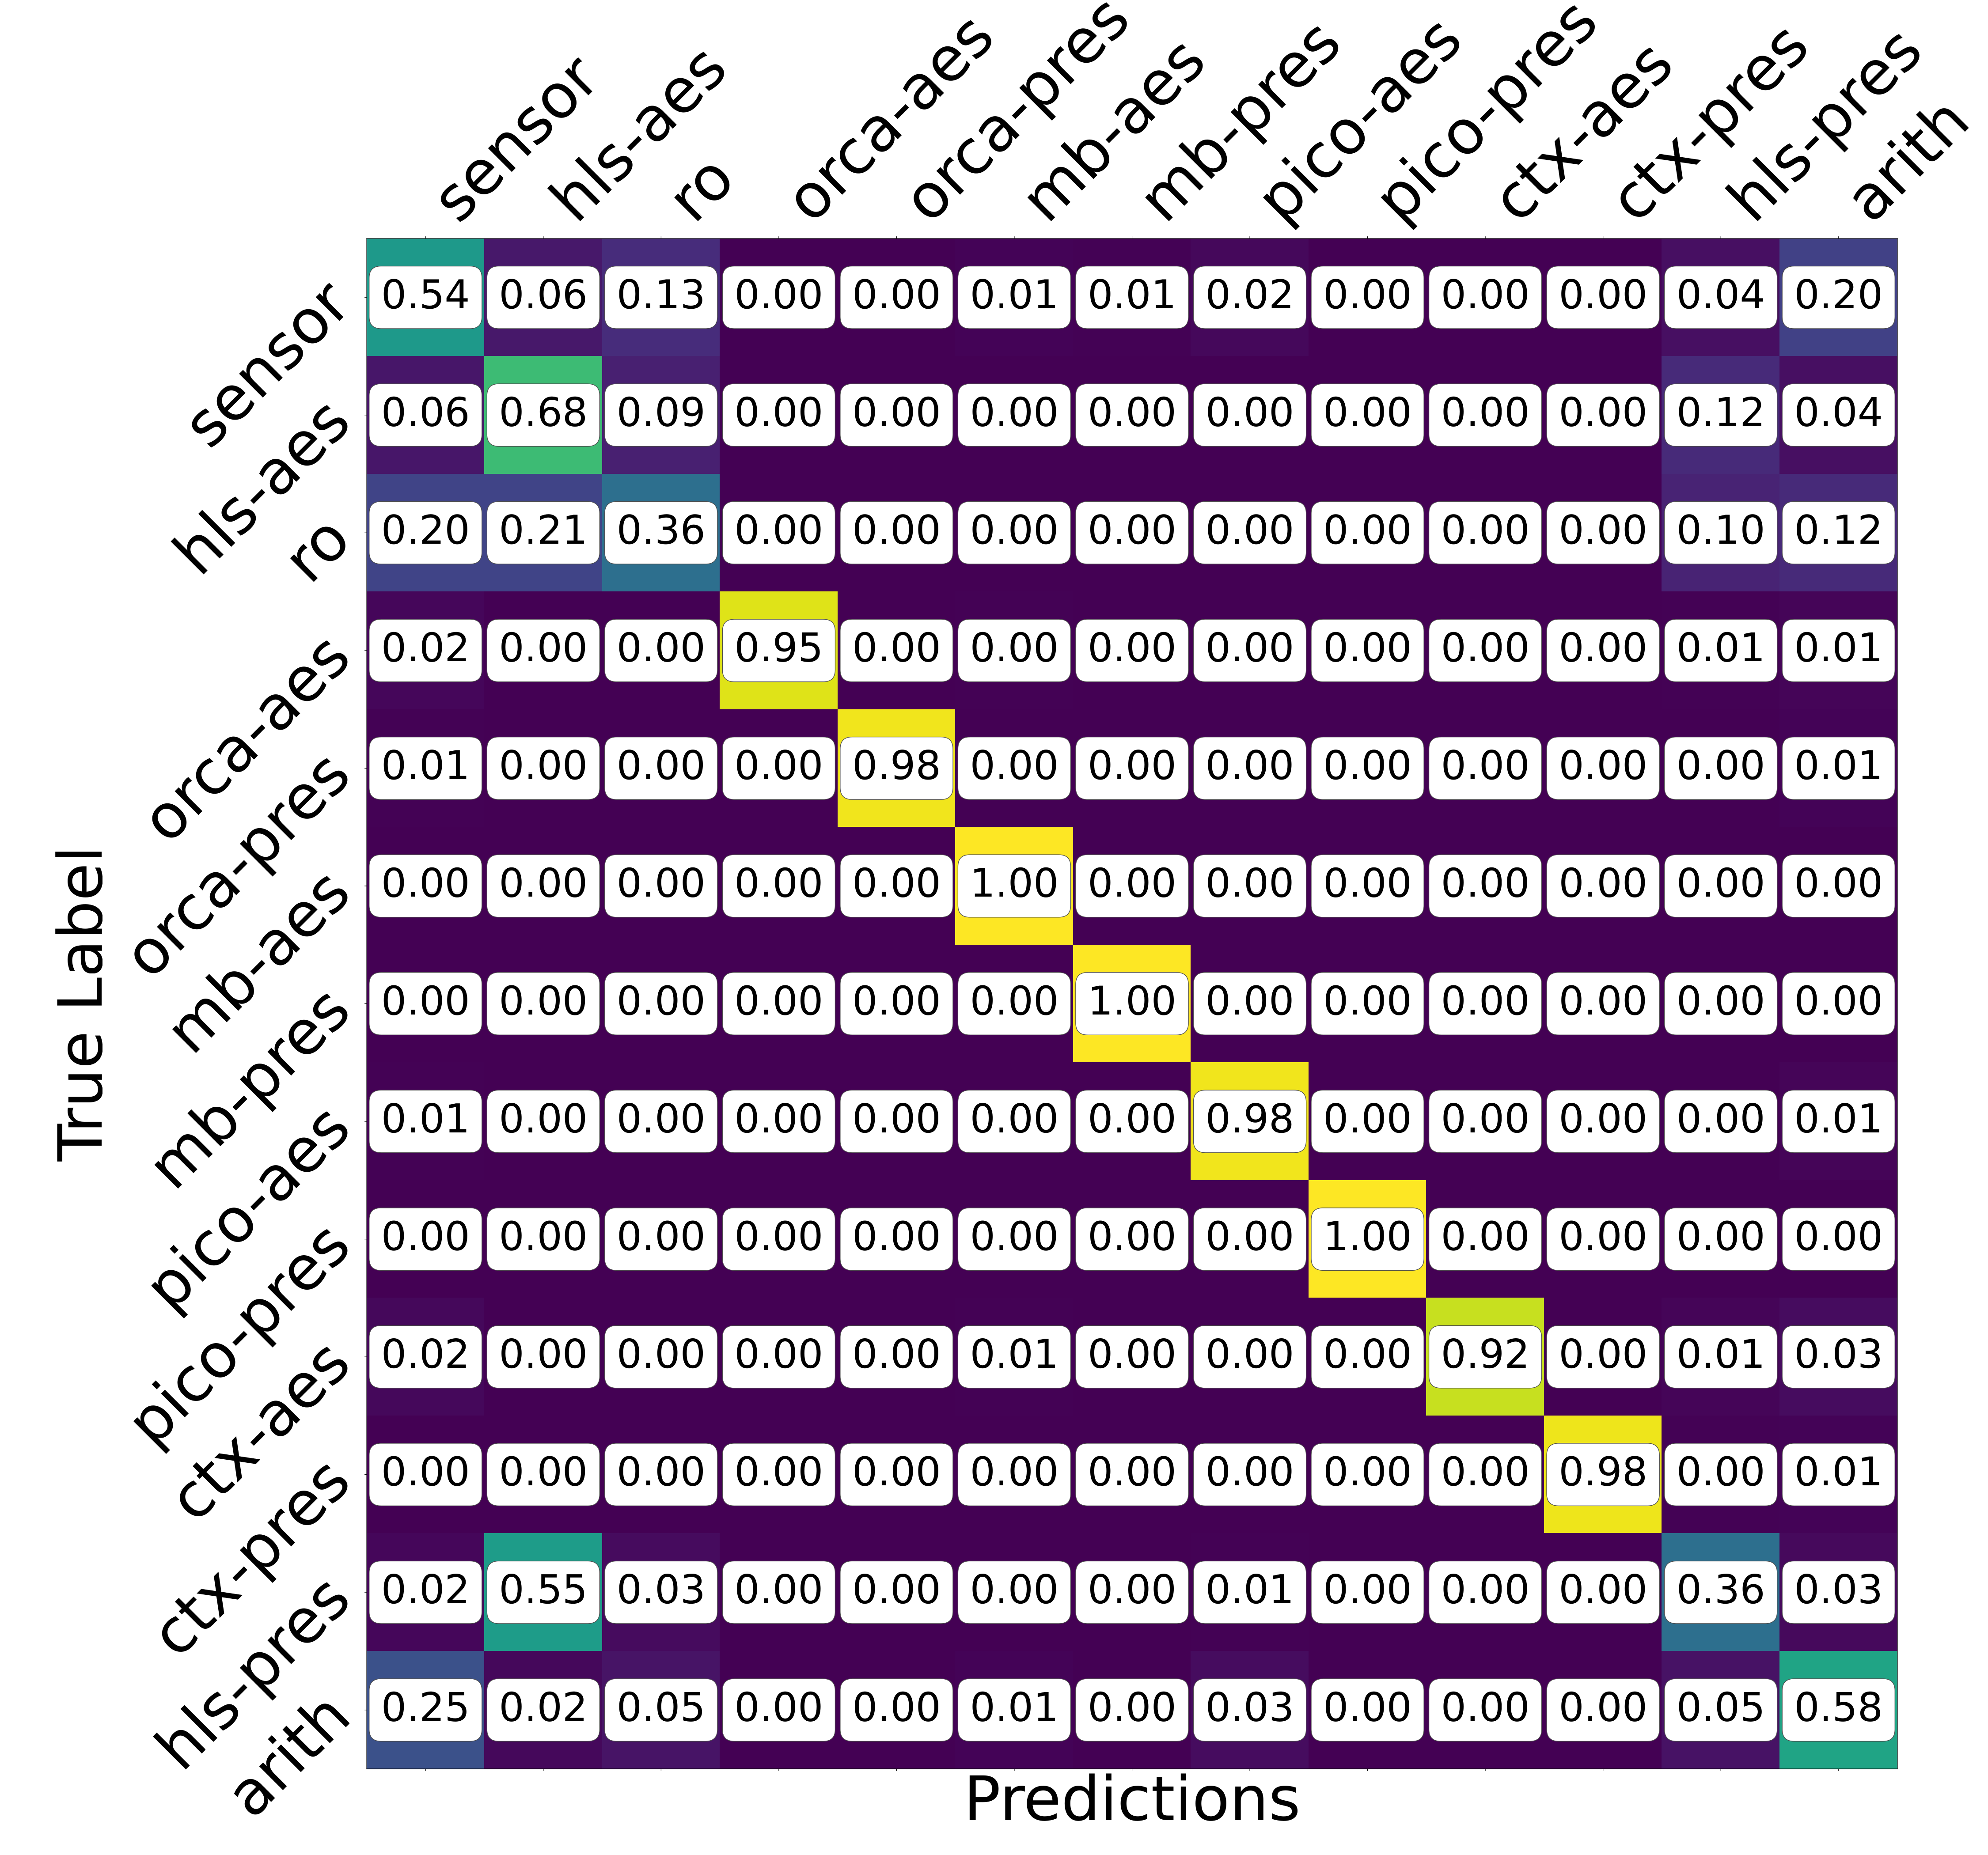
\includegraphics[scale=.043]{img/neg-backsub-maxphi-maxtheta-test-board_fd-big-text-confusion-matrix_trimmed.png}\label{classification/falling_max_max}}

% %\subfigure[($\downarrow\theta_{max}$, $\phi_{back}$)]{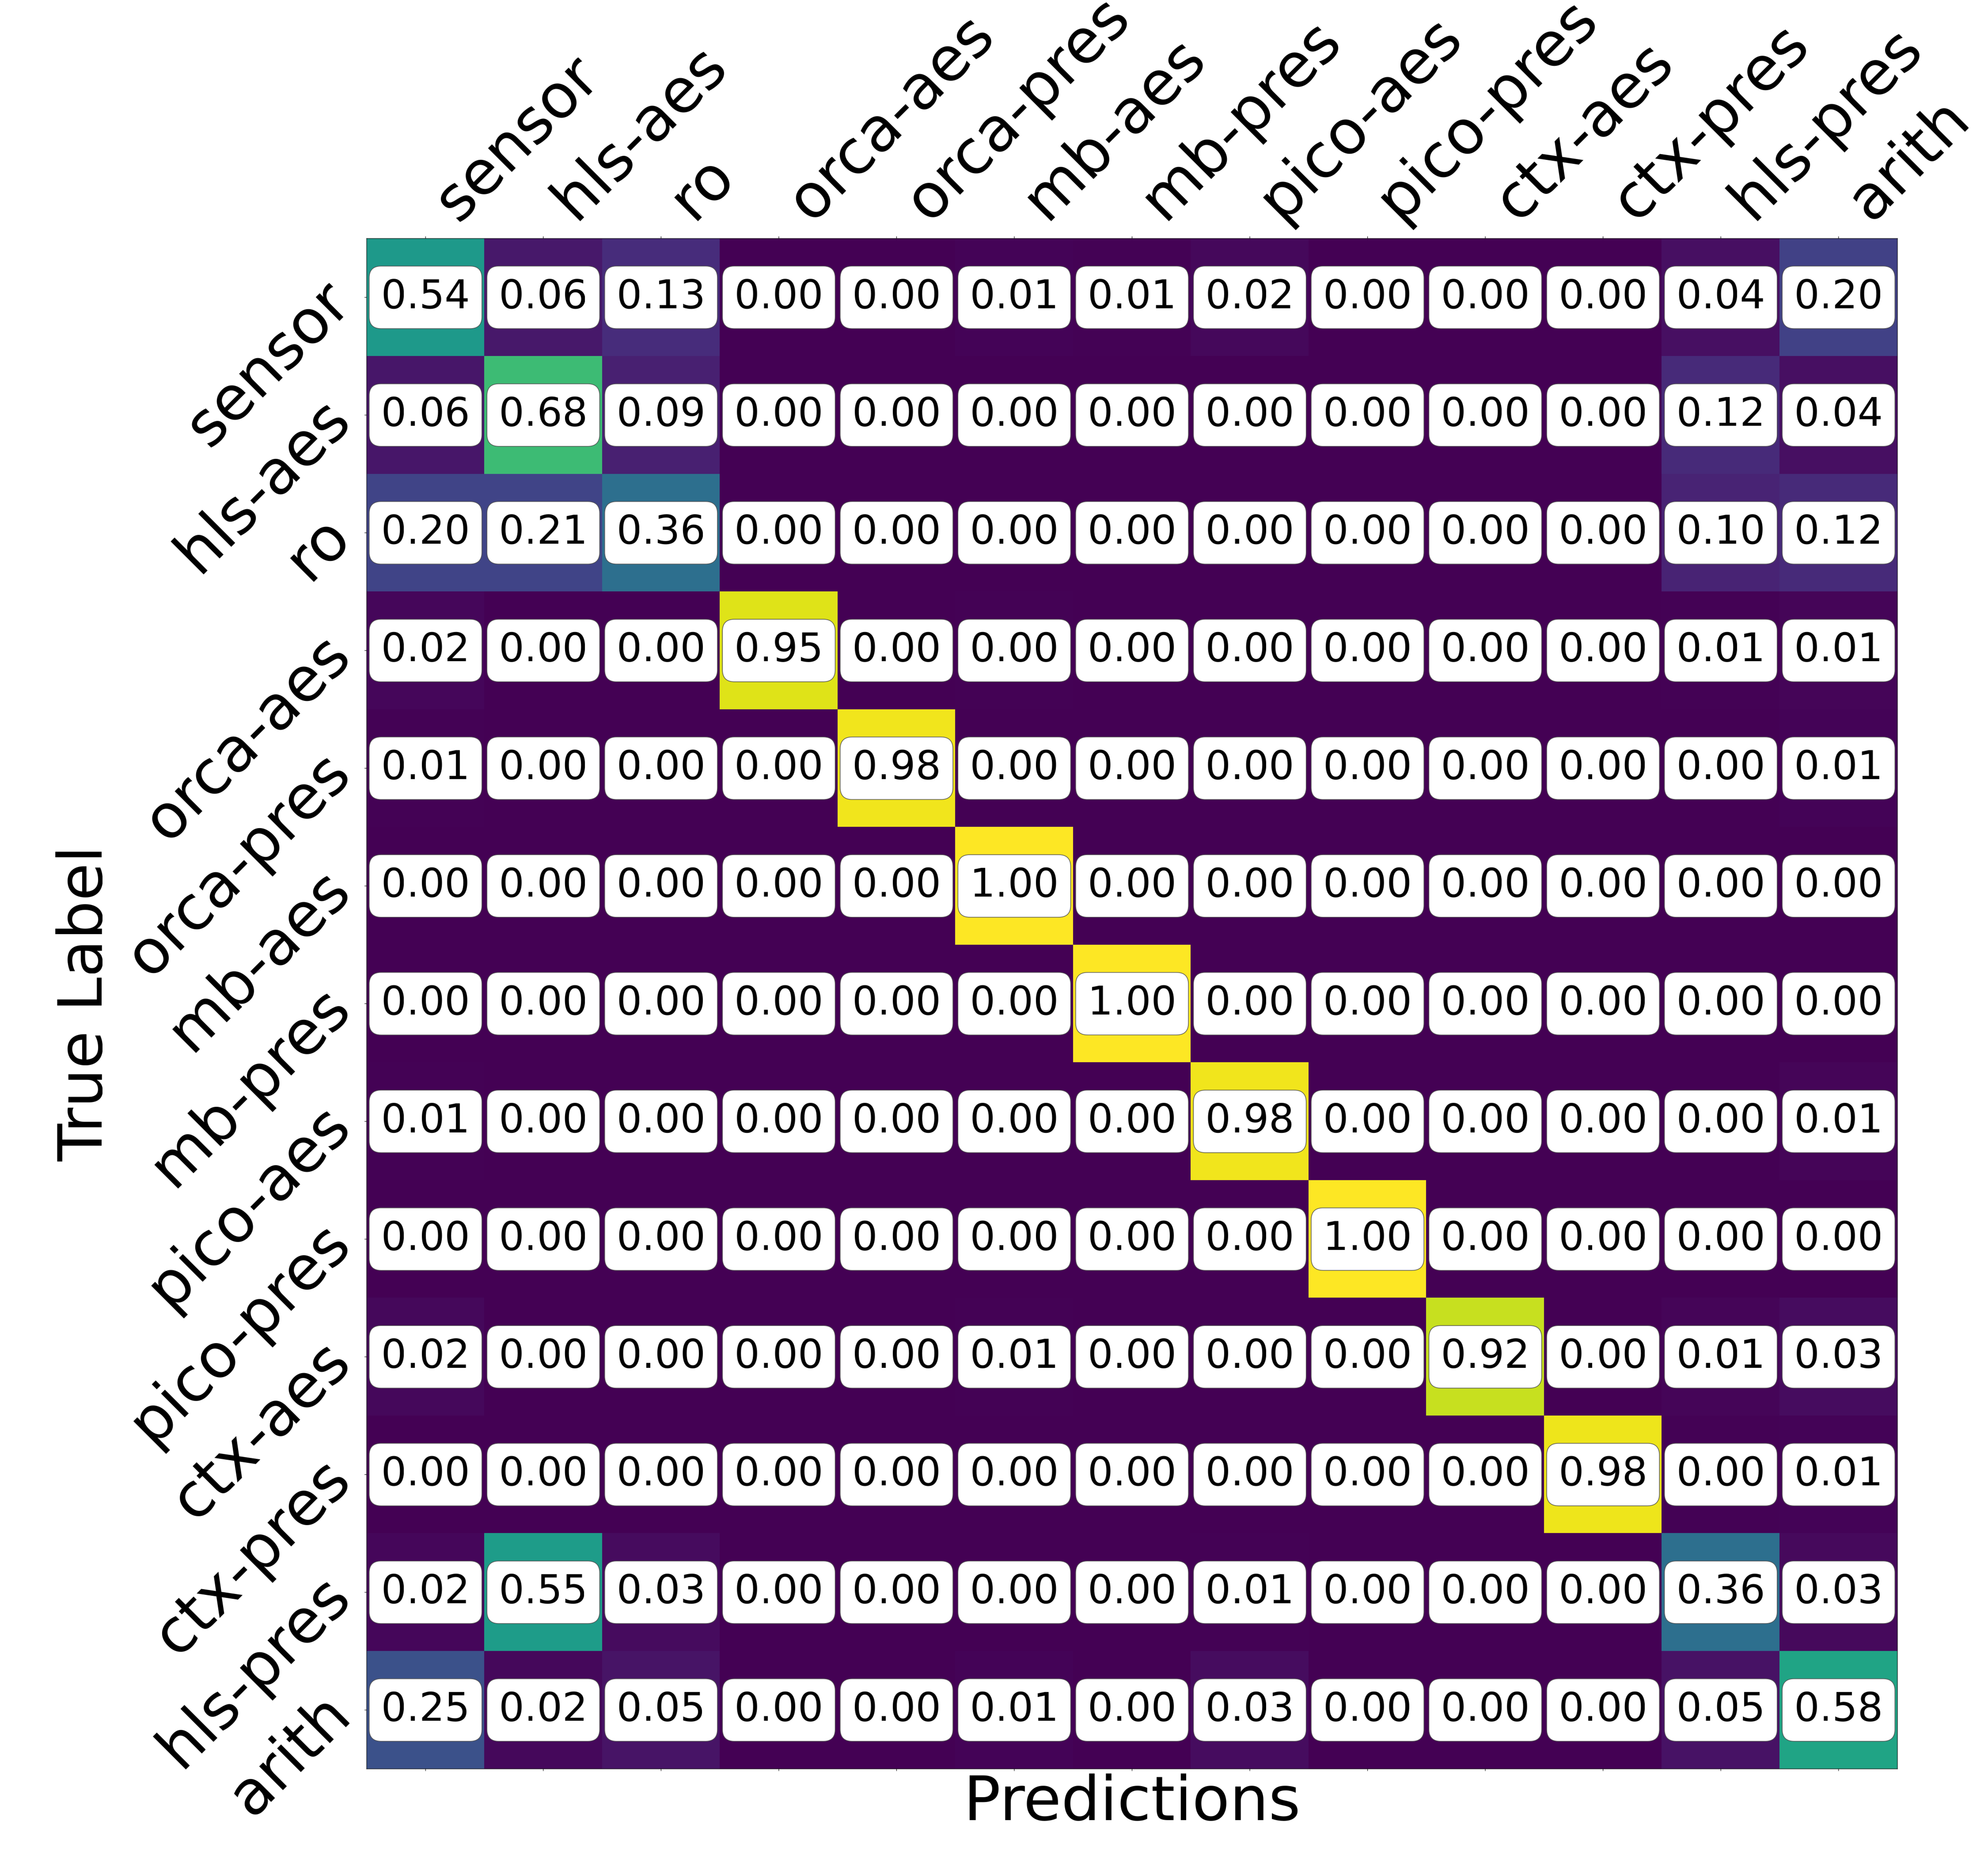
\includegraphics[scale=.09]{img/neg-backsub-maxphi-maxtheta-test-board_fd-big-text-confusion-matrix_trimmed.pdf}\label{classification/falling_max_max}} \\
% \vspace{-15px}
% \caption{Our \name TDC is employed in a 13-way classification task where an attacker extracts the type of co-located computation. The ability to  distinguish co-tenant computations is a measure of side-channel information contained in the sensor's traces.
% %The computations are introduced in Section~\ref{applications}.
% \ref{classification/rising_min_min} represents the worst-case where a TDC cannot reconfigure $\phi$ and $\theta$ and achieves 32\% accuracy. In \ref{classification/falling_min_max} the TDC can tune $\theta$ and improves to 51\% accuracy. In \ref{classification/falling_max_max} both $\theta$ and $\phi$ have been tuned with background subtraction to isolate co-tenant information and achieve 75\% accuracy, a 2.3$\times$ improvement. %\cd{Increase text size if possible. Reduce sig digits if needed}
% }%
% \label{fig:classification-main-figure}%
% \vspace{-10pt}%
% \end{figure*}%

\begin{figure*}[t!]

\begin{minipage}{.5\linewidth}
\centering
\subfloat[\hspace{15pt}($\uparrow\theta_{min}$, $\phi_{min}$): 32\% accuracy, Baseline]{\label{classification/rising_min_min}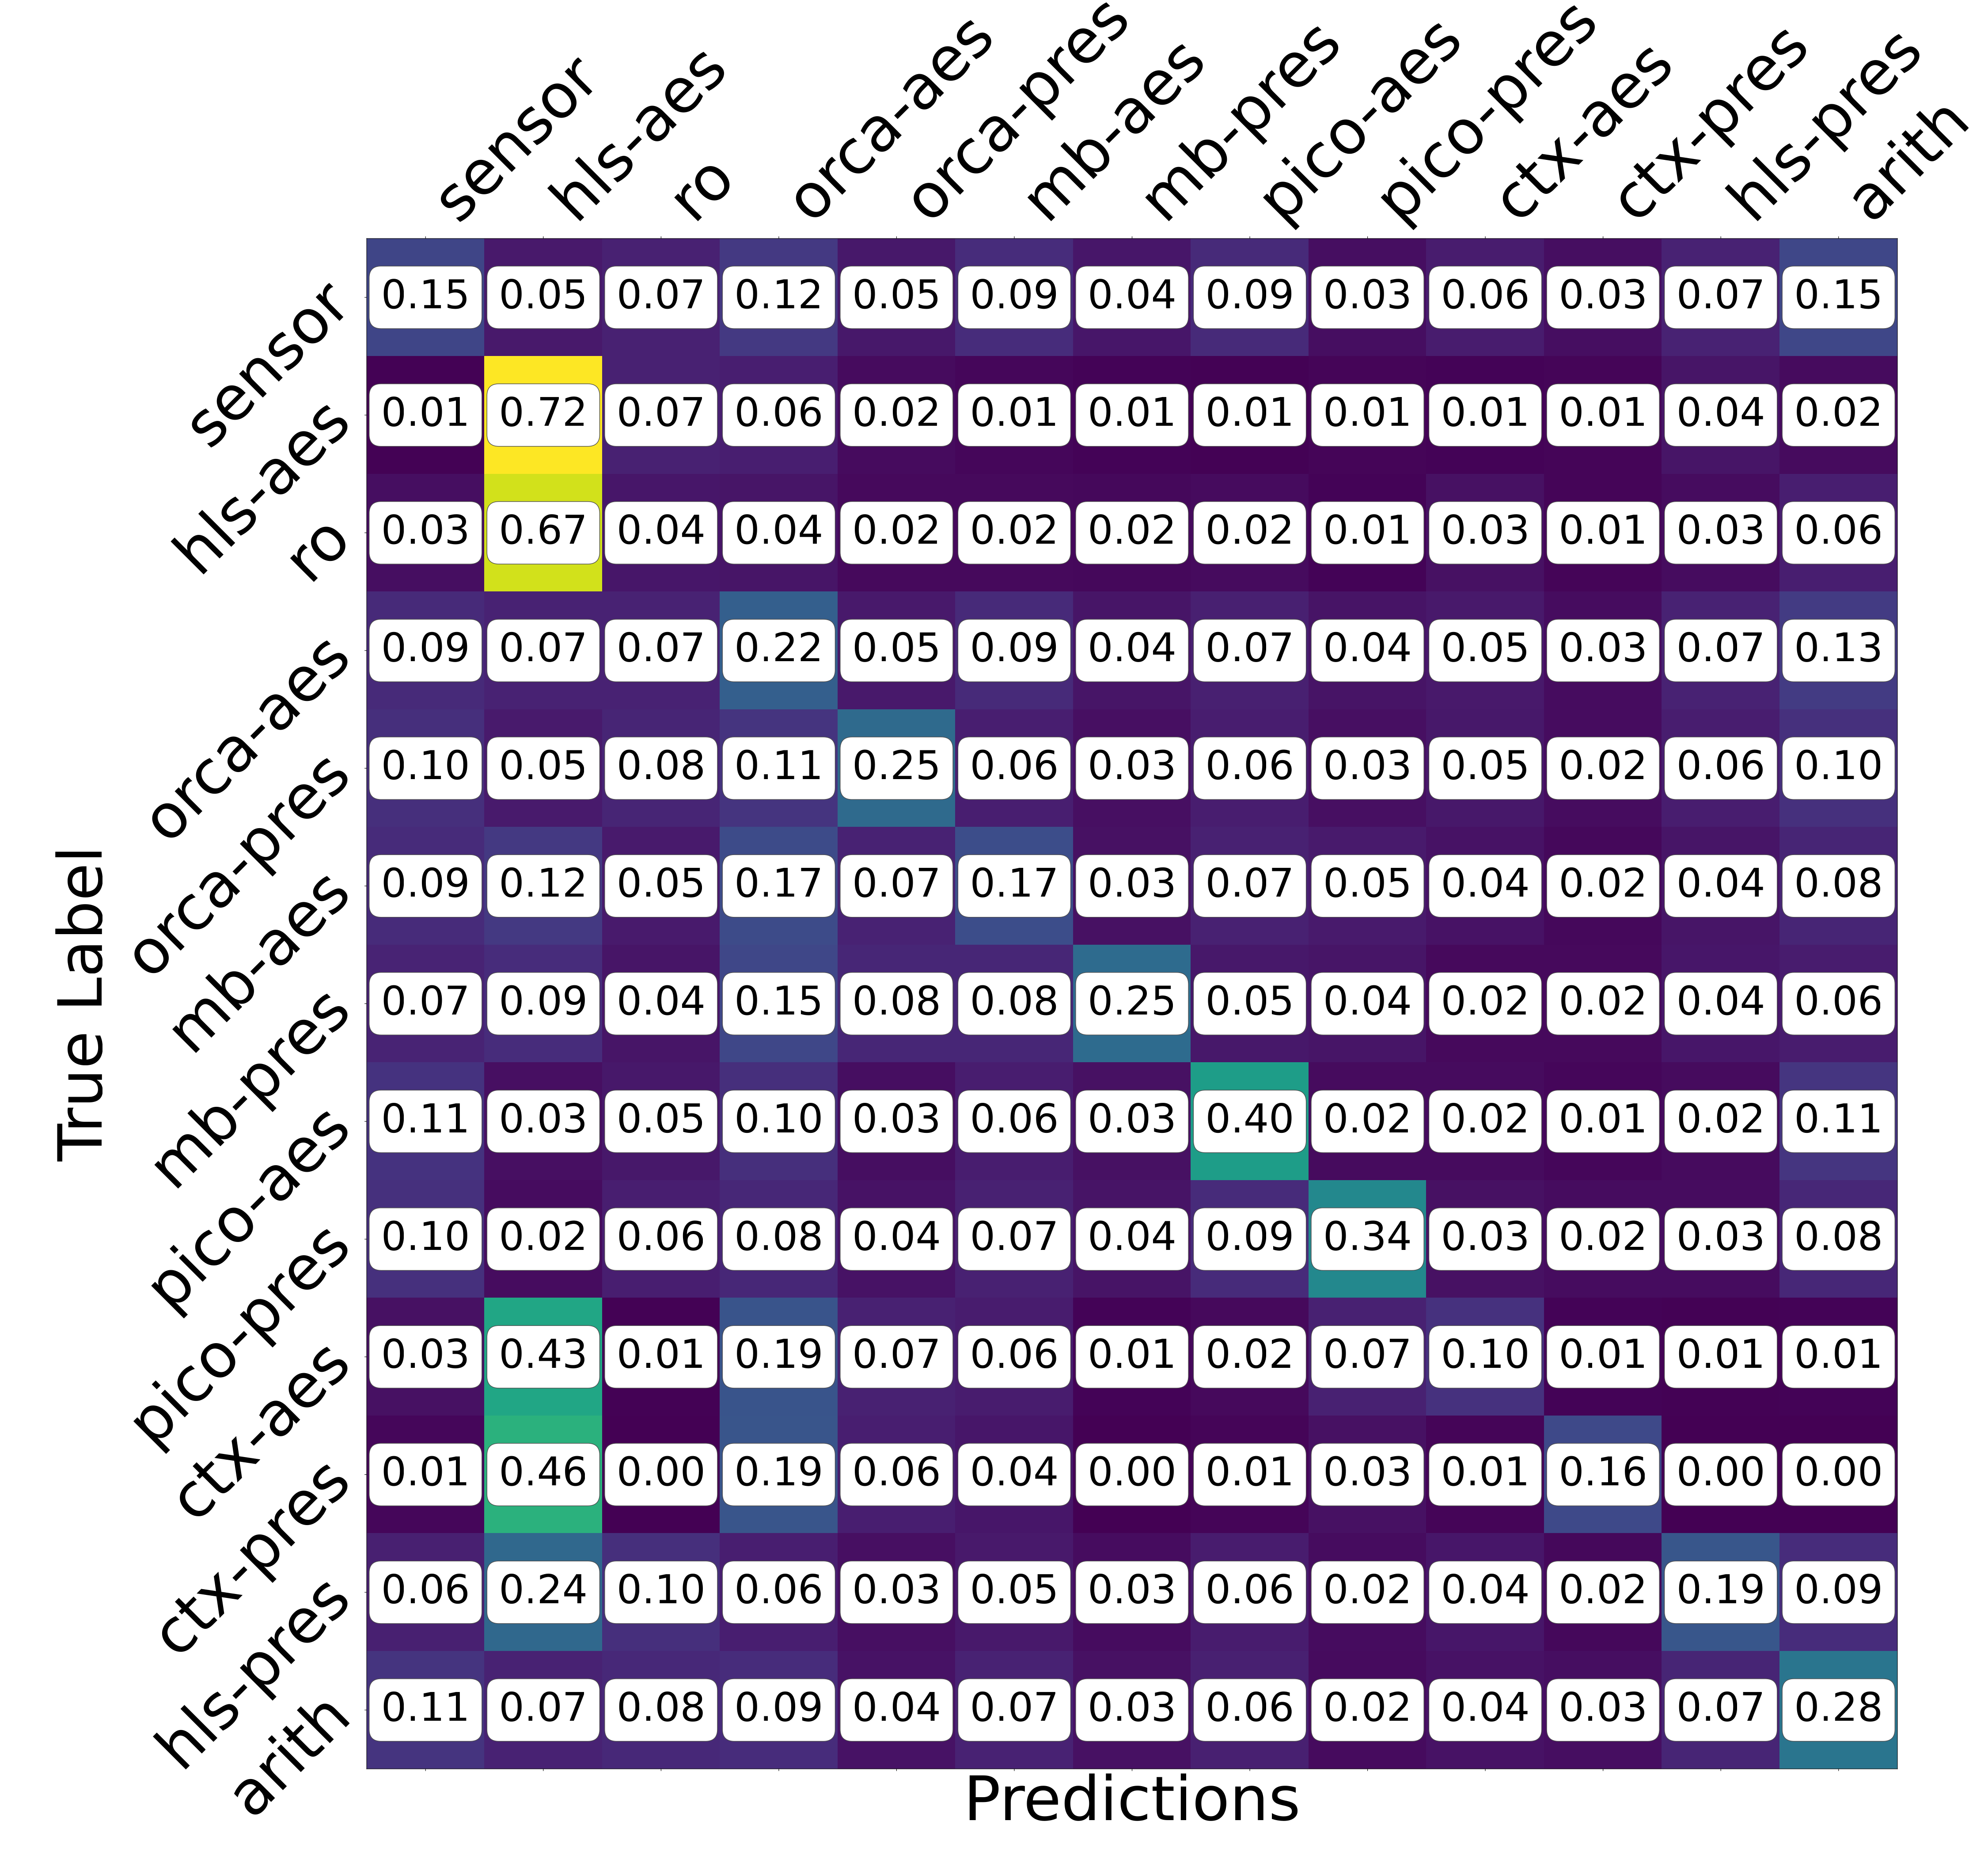
\includegraphics[width=.90\linewidth]{img/pos-minphi-mintheta-test-board_2e-big-text-confusion-matrix_trimmed.png}}
\end{minipage}%
\begin{minipage}{.5\linewidth}
\centering
\subfloat[\hspace{15pt}($\downarrow\theta_{max}$, $\phi_{min}$): 51\% accuracy, 1.6$\times$]{\label{classification/falling_min_max}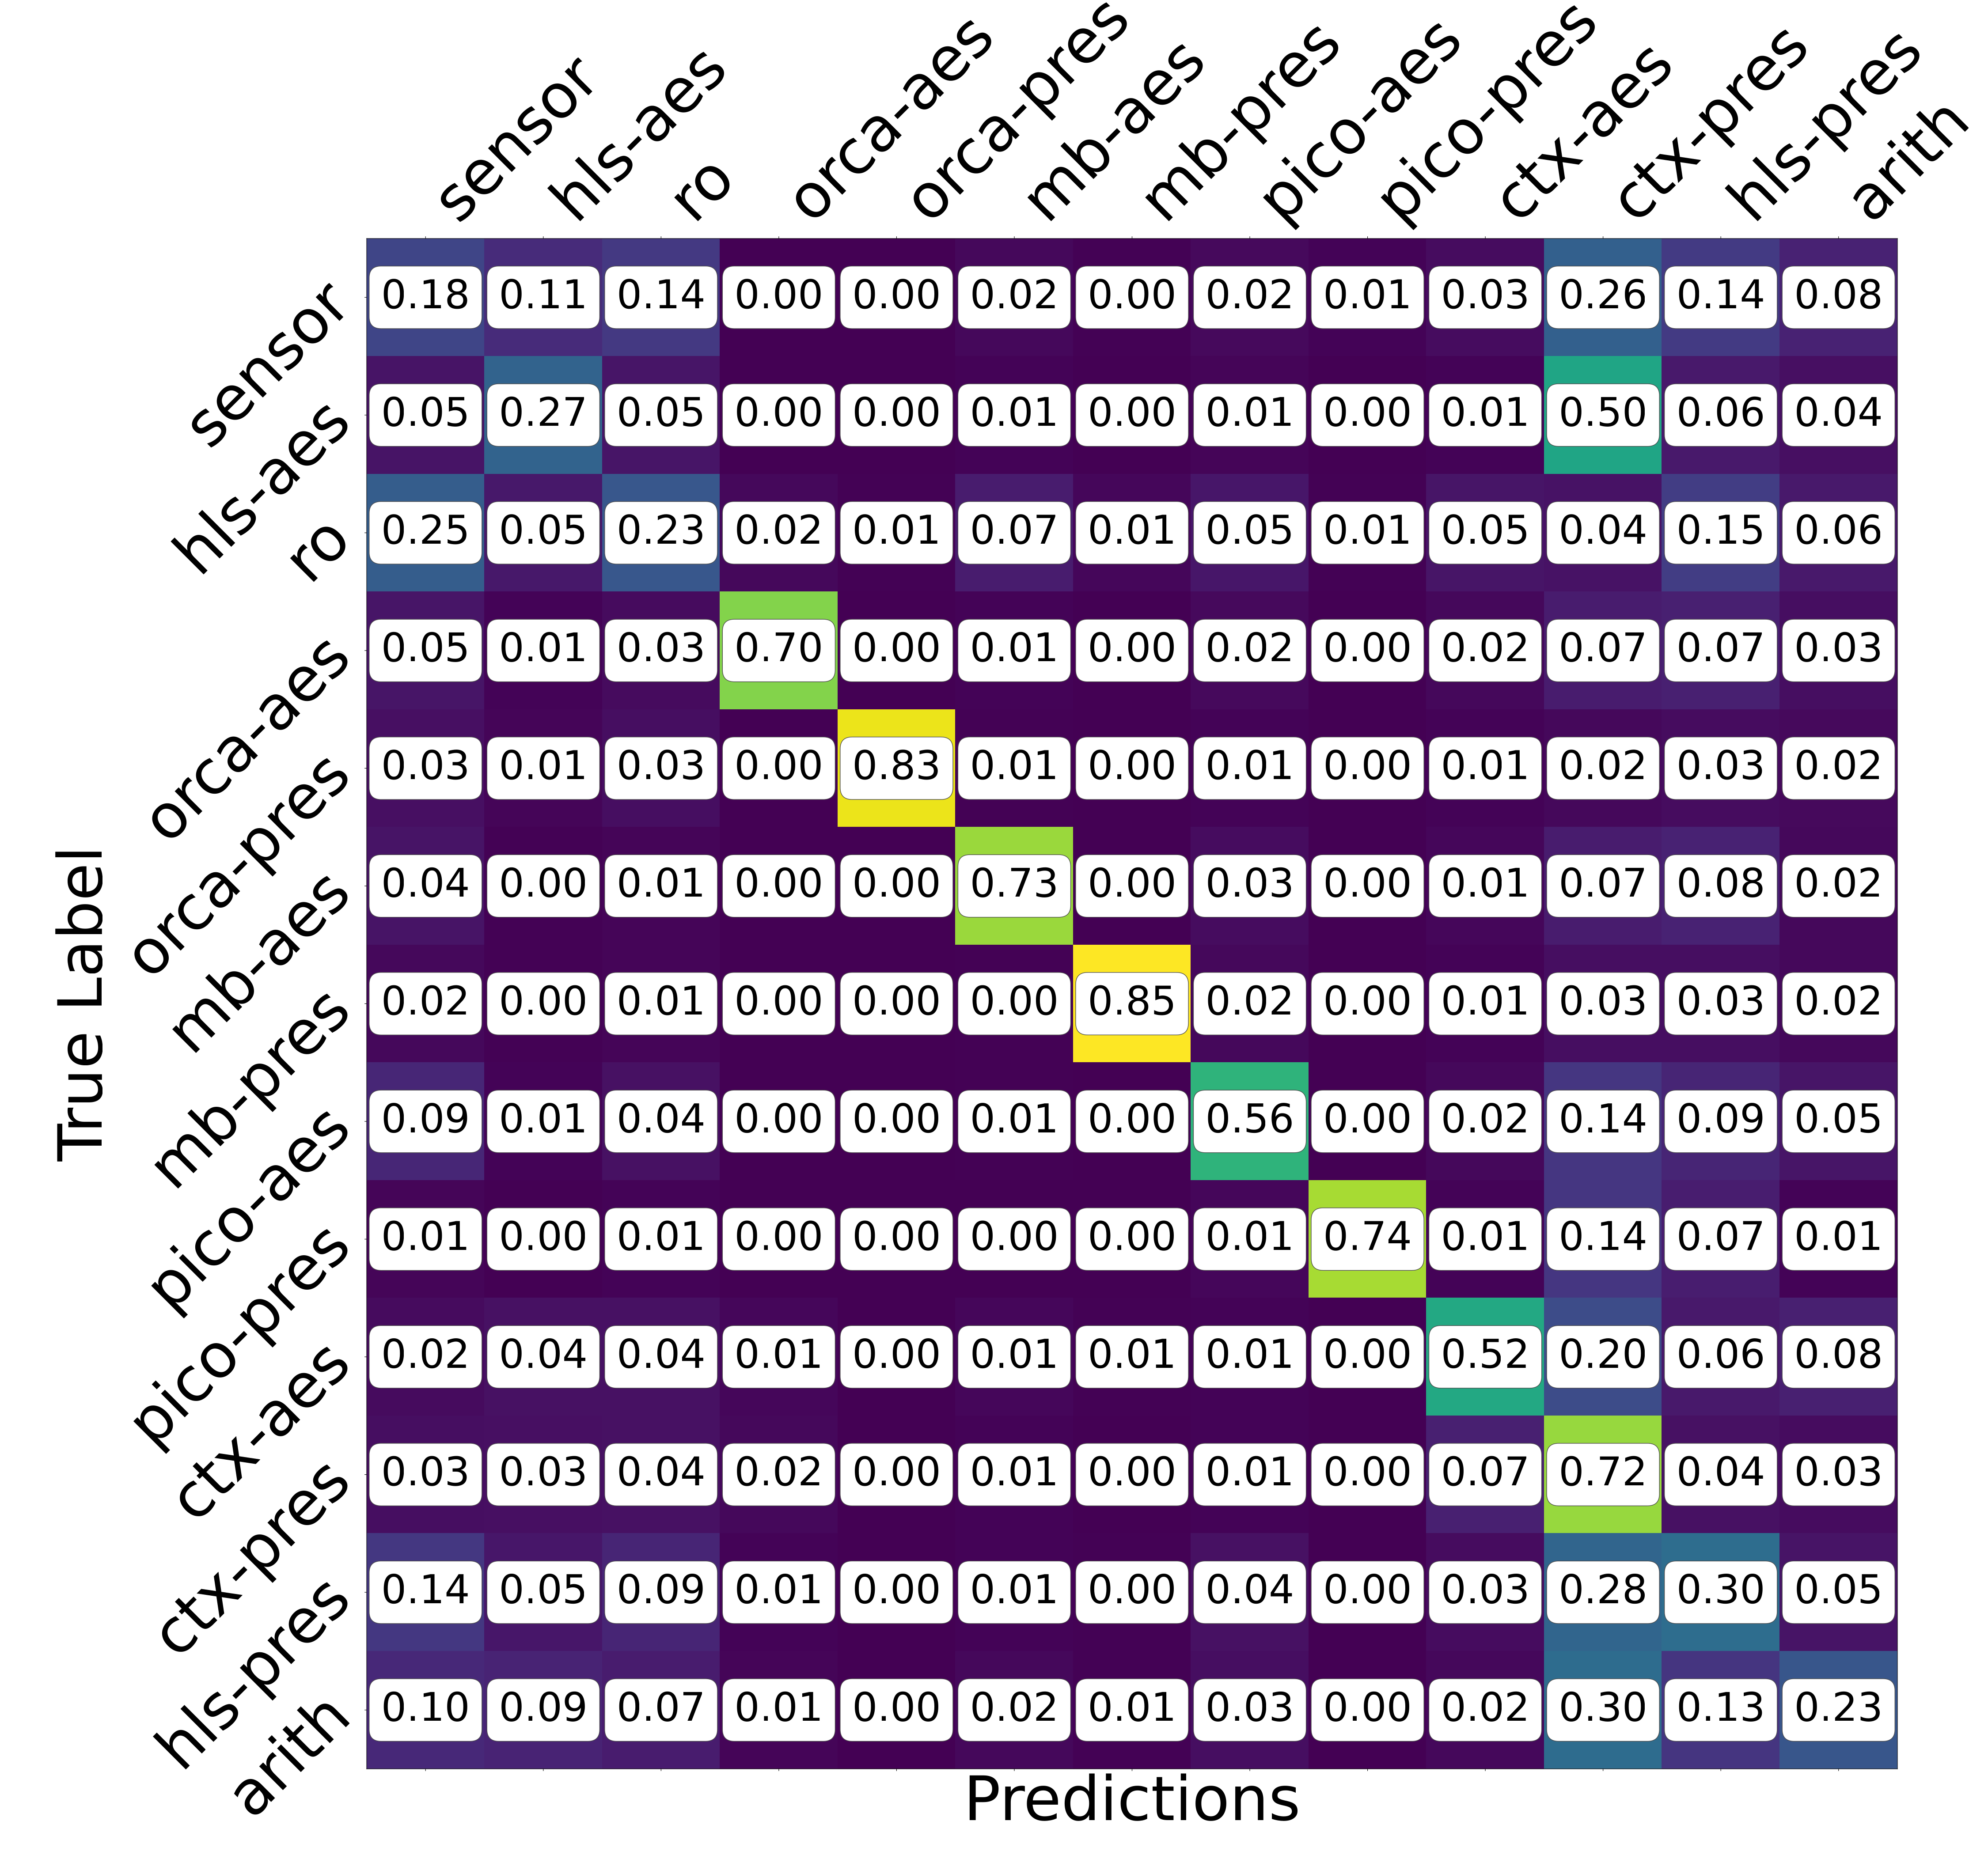
\includegraphics[width=.90\linewidth]{img/neg-minphi-mintheta-test-board_2e-big-text-confusion-matrix_trimmed.png}}
\end{minipage}\par\medskip
\centering
\subfloat[\hspace{15pt}$\downarrow\theta_{max}$, $\phi_{back}$): 75\% accuracy, 2.3$\times$]{\label{classification/falling_max_max}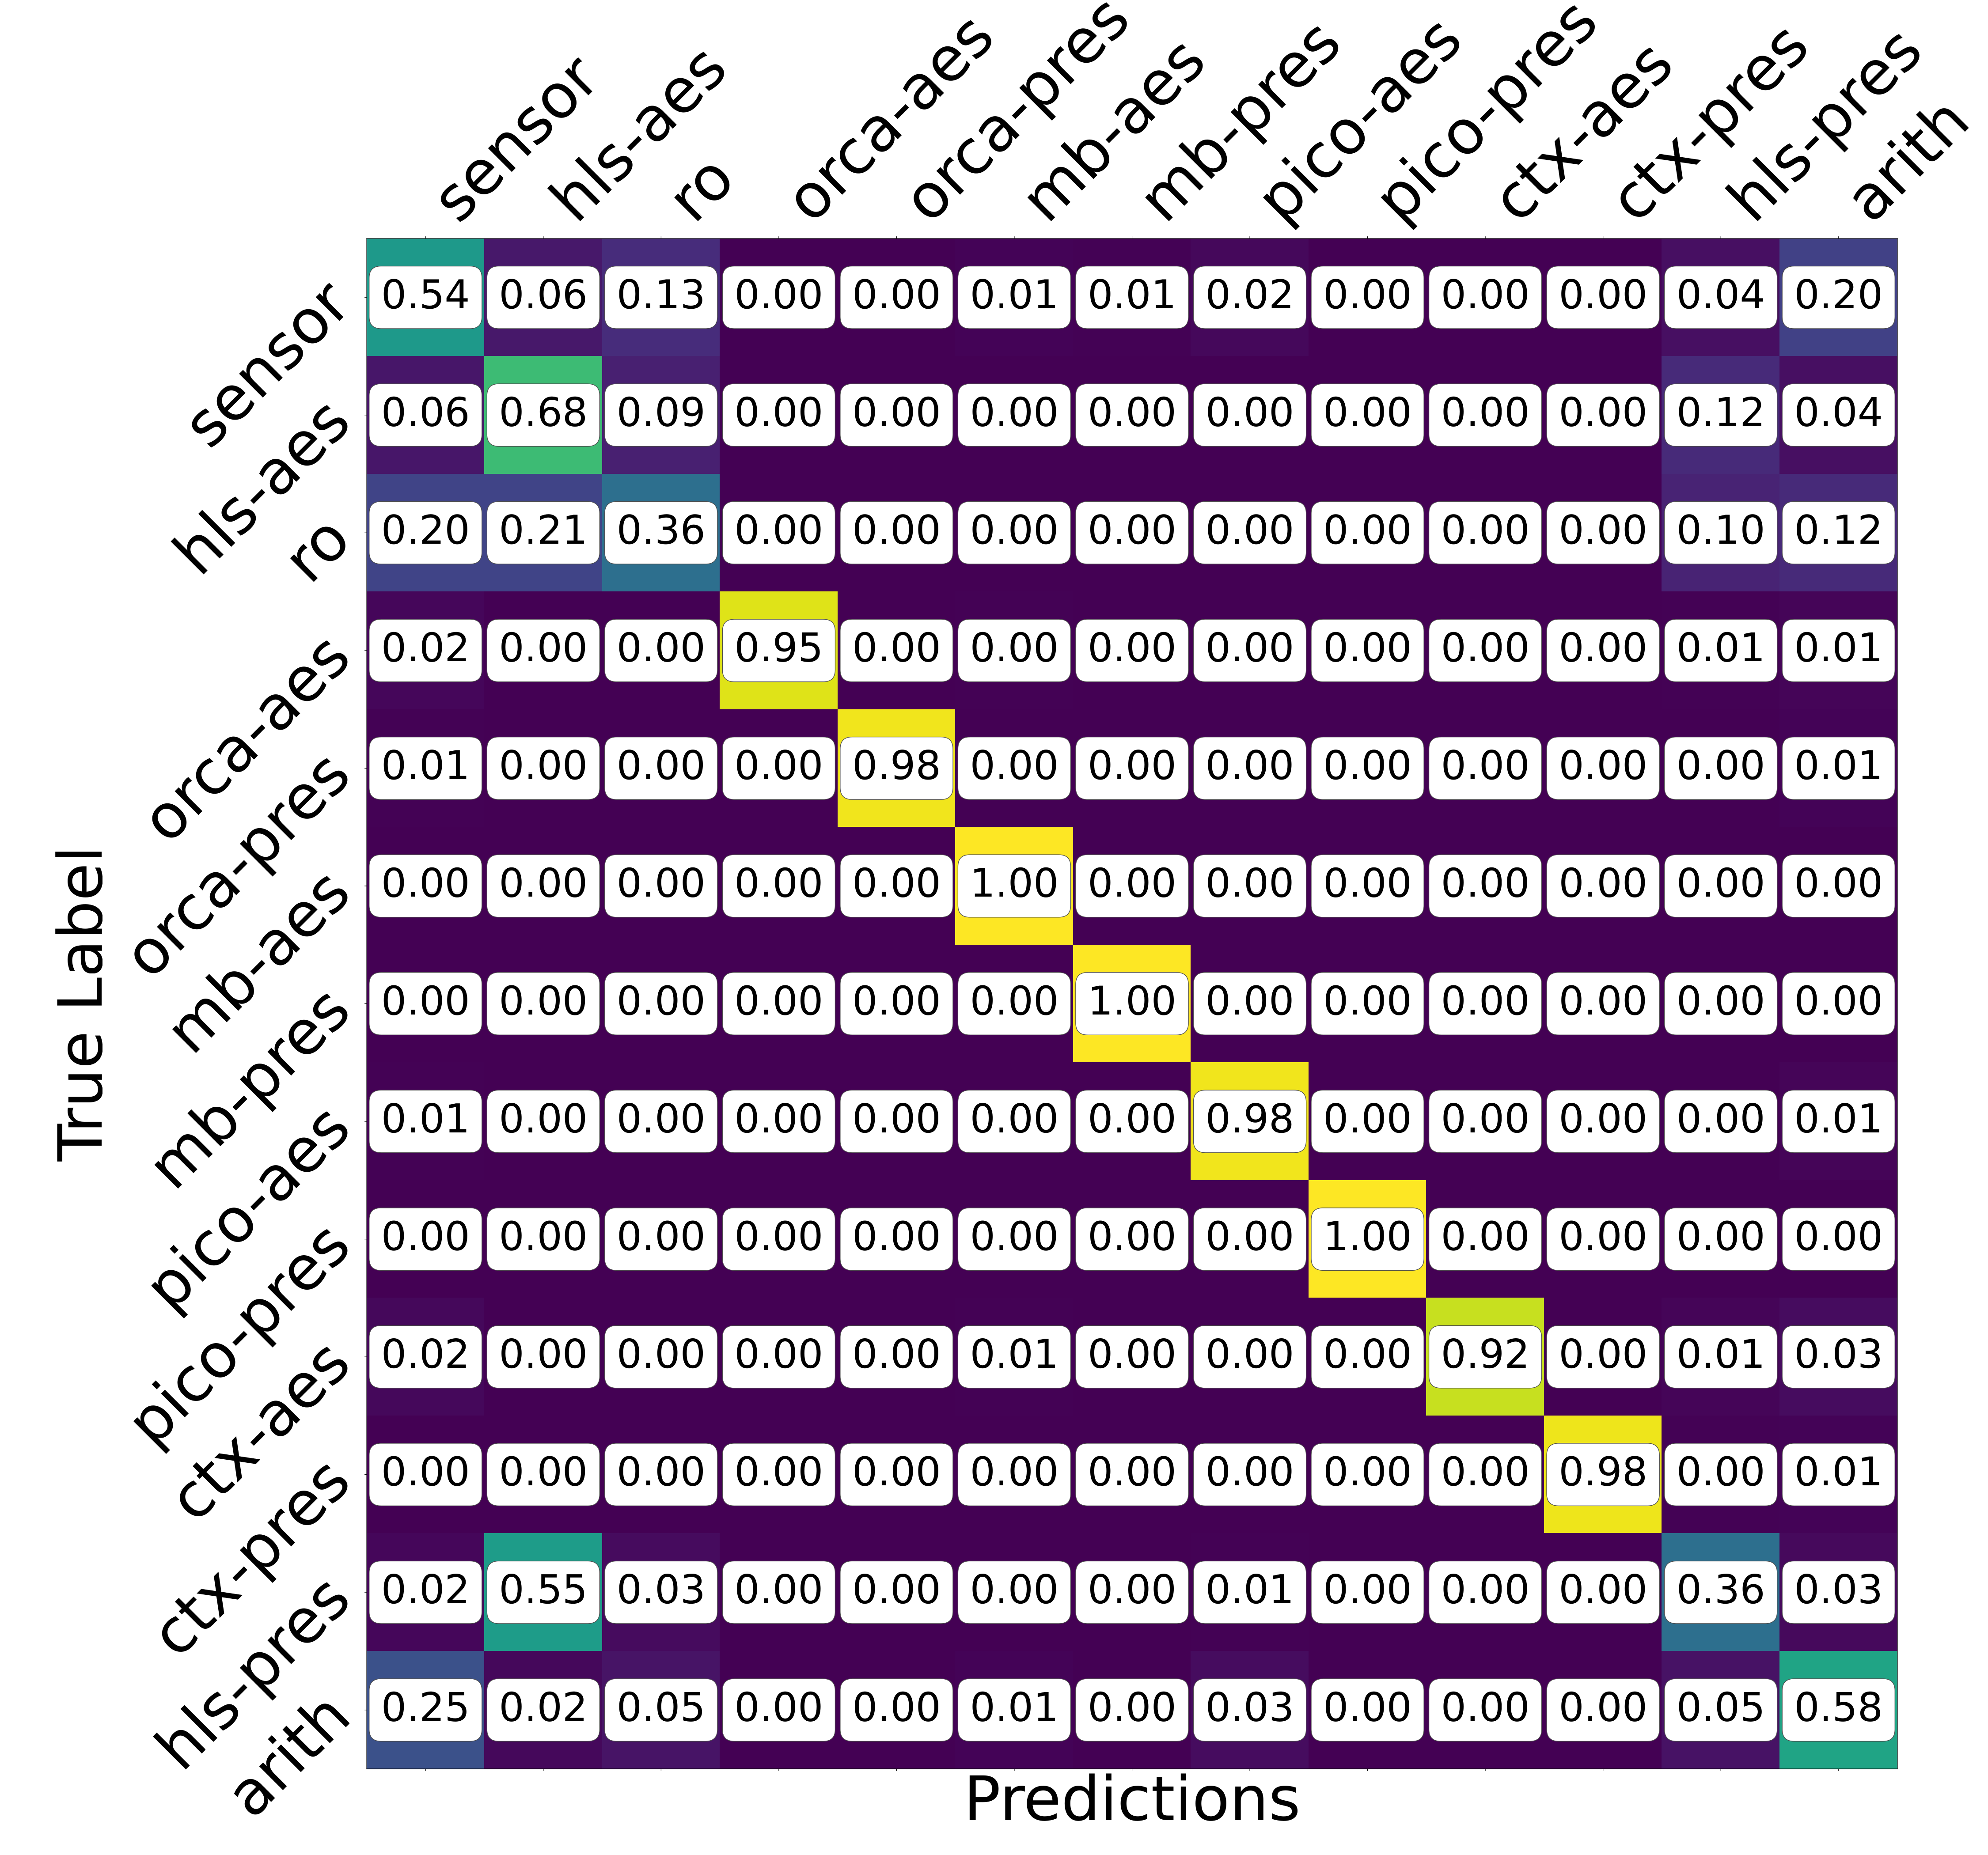
\includegraphics[width=.45\linewidth]{img/neg-backsub-maxphi-maxtheta-test-board_fd-big-text-confusion-matrix_trimmed.png}}

\caption{Our \name TDC is employed in a 13-way classification task where an attacker extracts the type of co-located computation. The ability to  distinguish co-tenant computations is a measure of side-channel information contained in the sensor's traces. The computations are introduced in Section~\ref{applications}. \ref{classification/rising_min_min} represents the worst-case where a TDC cannot reconfigure $\phi$ and $\theta$ and achieves 32\% accuracy. In \ref{classification/falling_min_max} the TDC can tune $\theta$ and improves to 51\% accuracy. In \ref{classification/falling_max_max} both $\theta$ and $\phi$ have been tuned with background subtraction to isolate co-tenant information and achieve 75\% accuracy, a 2.3$\times$ improvement.}
\vspace{-12px}
\label{fig:classification-main-figure}
\end{figure*}